\documentclass[openany]{book}
\usepackage{lmodern}
\usepackage{amssymb,amsmath}
\usepackage{ifxetex,ifluatex}
\usepackage{fixltx2e} % provides \textsubscript
\ifnum 0\ifxetex 1\fi\ifluatex 1\fi=0 % if pdftex
  \usepackage[T1]{fontenc}
  \usepackage[utf8]{inputenc}
\else % if luatex or xelatex
  \ifxetex
    \usepackage{mathspec}
  \else
    \usepackage{fontspec}
  \fi
  \defaultfontfeatures{Ligatures=TeX,Scale=MatchLowercase}
\fi
% use upquote if available, for straight quotes in verbatim environments
\IfFileExists{upquote.sty}{\usepackage{upquote}}{}
% use microtype if available
\IfFileExists{microtype.sty}{%
\usepackage{microtype}
\UseMicrotypeSet[protrusion]{basicmath} % disable protrusion for tt fonts
}{}
\usepackage[margin=1in]{geometry}
\usepackage{hyperref}
\hypersetup{unicode=true,
            pdftitle={DATA 624: Project 1},
            pdfauthor={Juliann McEachern},
            pdfborder={0 0 0},
            breaklinks=true}
\urlstyle{same}  % don't use monospace font for urls
\usepackage{natbib}
\bibliographystyle{plainnat}
\usepackage{color}
\usepackage{fancyvrb}
\newcommand{\VerbBar}{|}
\newcommand{\VERB}{\Verb[commandchars=\\\{\}]}
\DefineVerbatimEnvironment{Highlighting}{Verbatim}{commandchars=\\\{\}}
% Add ',fontsize=\small' for more characters per line
\usepackage{framed}
\definecolor{shadecolor}{RGB}{248,248,248}
\newenvironment{Shaded}{\begin{snugshade}}{\end{snugshade}}
\newcommand{\AlertTok}[1]{\textcolor[rgb]{0.94,0.16,0.16}{#1}}
\newcommand{\AnnotationTok}[1]{\textcolor[rgb]{0.56,0.35,0.01}{\textbf{\textit{#1}}}}
\newcommand{\AttributeTok}[1]{\textcolor[rgb]{0.77,0.63,0.00}{#1}}
\newcommand{\BaseNTok}[1]{\textcolor[rgb]{0.00,0.00,0.81}{#1}}
\newcommand{\BuiltInTok}[1]{#1}
\newcommand{\CharTok}[1]{\textcolor[rgb]{0.31,0.60,0.02}{#1}}
\newcommand{\CommentTok}[1]{\textcolor[rgb]{0.56,0.35,0.01}{\textit{#1}}}
\newcommand{\CommentVarTok}[1]{\textcolor[rgb]{0.56,0.35,0.01}{\textbf{\textit{#1}}}}
\newcommand{\ConstantTok}[1]{\textcolor[rgb]{0.00,0.00,0.00}{#1}}
\newcommand{\ControlFlowTok}[1]{\textcolor[rgb]{0.13,0.29,0.53}{\textbf{#1}}}
\newcommand{\DataTypeTok}[1]{\textcolor[rgb]{0.13,0.29,0.53}{#1}}
\newcommand{\DecValTok}[1]{\textcolor[rgb]{0.00,0.00,0.81}{#1}}
\newcommand{\DocumentationTok}[1]{\textcolor[rgb]{0.56,0.35,0.01}{\textbf{\textit{#1}}}}
\newcommand{\ErrorTok}[1]{\textcolor[rgb]{0.64,0.00,0.00}{\textbf{#1}}}
\newcommand{\ExtensionTok}[1]{#1}
\newcommand{\FloatTok}[1]{\textcolor[rgb]{0.00,0.00,0.81}{#1}}
\newcommand{\FunctionTok}[1]{\textcolor[rgb]{0.00,0.00,0.00}{#1}}
\newcommand{\ImportTok}[1]{#1}
\newcommand{\InformationTok}[1]{\textcolor[rgb]{0.56,0.35,0.01}{\textbf{\textit{#1}}}}
\newcommand{\KeywordTok}[1]{\textcolor[rgb]{0.13,0.29,0.53}{\textbf{#1}}}
\newcommand{\NormalTok}[1]{#1}
\newcommand{\OperatorTok}[1]{\textcolor[rgb]{0.81,0.36,0.00}{\textbf{#1}}}
\newcommand{\OtherTok}[1]{\textcolor[rgb]{0.56,0.35,0.01}{#1}}
\newcommand{\PreprocessorTok}[1]{\textcolor[rgb]{0.56,0.35,0.01}{\textit{#1}}}
\newcommand{\RegionMarkerTok}[1]{#1}
\newcommand{\SpecialCharTok}[1]{\textcolor[rgb]{0.00,0.00,0.00}{#1}}
\newcommand{\SpecialStringTok}[1]{\textcolor[rgb]{0.31,0.60,0.02}{#1}}
\newcommand{\StringTok}[1]{\textcolor[rgb]{0.31,0.60,0.02}{#1}}
\newcommand{\VariableTok}[1]{\textcolor[rgb]{0.00,0.00,0.00}{#1}}
\newcommand{\VerbatimStringTok}[1]{\textcolor[rgb]{0.31,0.60,0.02}{#1}}
\newcommand{\WarningTok}[1]{\textcolor[rgb]{0.56,0.35,0.01}{\textbf{\textit{#1}}}}
\usepackage{graphicx,grffile}
\makeatletter
\def\maxwidth{\ifdim\Gin@nat@width>\linewidth\linewidth\else\Gin@nat@width\fi}
\def\maxheight{\ifdim\Gin@nat@height>\textheight\textheight\else\Gin@nat@height\fi}
\makeatother
% Scale images if necessary, so that they will not overflow the page
% margins by default, and it is still possible to overwrite the defaults
% using explicit options in \includegraphics[width, height, ...]{}
\setkeys{Gin}{width=\maxwidth,height=\maxheight,keepaspectratio}
\IfFileExists{parskip.sty}{%
\usepackage{parskip}
}{% else
\setlength{\parindent}{0pt}
\setlength{\parskip}{6pt plus 2pt minus 1pt}
}
\setlength{\emergencystretch}{3em}  % prevent overfull lines
\providecommand{\tightlist}{%
  \setlength{\itemsep}{0pt}\setlength{\parskip}{0pt}}
\setcounter{secnumdepth}{5}

%%% Use protect on footnotes to avoid problems with footnotes in titles
\let\rmarkdownfootnote\footnote%
\def\footnote{\protect\rmarkdownfootnote}

%%% Change title format to be more compact
\usepackage{titling}

% Create subtitle command for use in maketitle
\providecommand{\subtitle}[1]{
  \posttitle{
    \begin{center}\large#1\end{center}
    }
}

\setlength{\droptitle}{-2em}

  \title{DATA 624: Project 1}
    \pretitle{\vspace{\droptitle}\centering\huge}
  \posttitle{\par}
    \author{Juliann McEachern}
    \preauthor{\centering\large\emph}
  \postauthor{\par}
      \predate{\centering\large\emph}
  \postdate{\par}
    \date{October 22, 2019}

\usepackage{booktabs}
\usepackage[table]{xcolor}

% set plain style for page numbers
\pagestyle{plain}
\raggedbottom

% change font
\usepackage{fontspec}
\setmainfont{Arial}

% remove "chapter" from chapter title
\usepackage{titlesec}
\titleformat{\chapter}
  {\normalfont\LARGE\bfseries}{\thechapter}{1em}{}
\titlespacing*{\chapter}{0pt}{3.5ex plus 1ex minus .2ex}{2.3ex plus .2ex}

% create color block quotes
\usepackage{tcolorbox}
\newtcolorbox{myquote}{colback=orange!05!white, colframe=black!75!black}
\renewenvironment{quote}{\begin{myquote}}{\end{myquote}}

% wrap text
\usepackage{geometry}[textwidth=6in]

% kable 
\usepackage{tabu}
\usepackage{float}
\usepackage{booktabs}
\usepackage{longtable}
\usepackage{array}
\usepackage{multirow}
\usepackage{wrapfig}
\usepackage{float}
\usepackage{colortbl}
\usepackage{pdflscape}
\usepackage{tabu}
\usepackage{threeparttable}
\usepackage{threeparttablex}
\usepackage[normalem]{ulem}
\usepackage{makecell}
\usepackage{xcolor}

\begin{document}
\maketitle

{
\setcounter{tocdepth}{1}
\tableofcontents
}
\hypertarget{overview}{%
\chapter*{Overview}\label{overview}}
\addcontentsline{toc}{chapter}{Overview}

\begin{quote}
I am leaving the project overview page here for us to compile our final
report in one singular document. We will add additional information here
regarding project one to include explanation of process, etc.
\end{quote}

\hypertarget{dependencies}{%
\section*{Dependencies}\label{dependencies}}
\addcontentsline{toc}{section}{Dependencies}

\begin{quote}
Please add all libraries used here.
\end{quote}

The following R libraries were used to complete Project 1:

\begin{Shaded}
\begin{Highlighting}[]
\CommentTok{# General}
\KeywordTok{library}\NormalTok{(}\StringTok{'easypackages'}\NormalTok{)}

\KeywordTok{libraries}\NormalTok{(}\StringTok{'knitr'}\NormalTok{, }\StringTok{'kableExtra'}\NormalTok{, }\StringTok{'default'}\NormalTok{)}

\CommentTok{# Processing}
\KeywordTok{libraries}\NormalTok{(}\StringTok{'readxl'}\NormalTok{, }\StringTok{'tidyverse'}\NormalTok{, }\StringTok{'janitor'}\NormalTok{, }\StringTok{'lubridate'}\NormalTok{)}

\CommentTok{# Graphing}
\KeywordTok{libraries}\NormalTok{(}\StringTok{'ggplot2'}\NormalTok{, }\StringTok{'grid'}\NormalTok{, }\StringTok{'gridExtra'}\NormalTok{)}

\CommentTok{# Timeseries }
\KeywordTok{libraries}\NormalTok{(}\StringTok{'zoo'}\NormalTok{, }\StringTok{'urca'}\NormalTok{, }\StringTok{'tseries'}\NormalTok{, }\StringTok{'timetk'}\NormalTok{)}

\CommentTok{# Math}
\KeywordTok{libraries}\NormalTok{(}\StringTok{'forecast'}\NormalTok{)}
\end{Highlighting}
\end{Shaded}

\hypertarget{data}{%
\section*{Data}\label{data}}
\addcontentsline{toc}{section}{Data}

Data was stored within our group repository and imported below using the
\texttt{readxl} package. Each individual question was solved within an R
script and the data was sourced into our main report for discussion
purposes. The R scripts are available within our appendix for
replication purposes.

For grading purposes, we exported and saved all forecasts as a csv in
our data folder.

\begin{Shaded}
\begin{Highlighting}[]
\CommentTok{# Data Aquisition}
\NormalTok{atm_data <-}\StringTok{ }\KeywordTok{read_excel}\NormalTok{(}\StringTok{"data/ATM624Data.xlsx"}\NormalTok{) }
\NormalTok{power_data <-}\StringTok{ }\KeywordTok{read_excel}\NormalTok{(}\StringTok{"data/ResidentialCustomerForecastLoad-624.xlsx"}\NormalTok{) }
\NormalTok{pipe1_data <-}\StringTok{ }\KeywordTok{read_excel}\NormalTok{(}\StringTok{"data/Waterflow_Pipe1.xlsx"}\NormalTok{)}
\NormalTok{pipe2_data <-}\StringTok{ }\KeywordTok{read_excel}\NormalTok{(}\StringTok{"data/Waterflow_Pipe2.xlsx"}\NormalTok{)}

\CommentTok{# Source Code}
\KeywordTok{source}\NormalTok{(}\StringTok{"scripts/Part-A-JM.R"}\NormalTok{)}
\end{Highlighting}
\end{Shaded}

\hypertarget{part-a}{%
\chapter{Part A}\label{part-a}}

\begin{quote}
\textbf{Instructions:} In part A, I want you to forecast how much cash
is taken out of 4 different ATM machines for May 2010. The data is given
in a single file. The variable \texttt{Cash} is provided in hundreds of
dollars, other than that it is straight forward. I am being somewhat
ambiguous on purpose. I am giving you data, please provide your written
report on your findings, visuals, discussion and your R code all within
a Word readable document, except the forecast which you will put in an
Excel readable file. I must be able to cut and paste your R code and run
it in R studio. Your report must be professional - most of all -
readable, EASY to follow. Let me know what you are thinking, assumptions
you are making! Your forecast is a simple CSV or Excel file that MATCHES
the format of the data I provide.
\end{quote}

\hypertarget{exploration}{%
\section{Exploration}\label{exploration}}

Through data exploration, we identified that the original data file
contained \texttt{NA} values in our \texttt{ATM} and \texttt{Cash}
columns for 14 observations in May 2010. We removed these missing values
and transformed the dataset into a wide format. Our cleaned dataframe
was then converted into a timeseries format using the \texttt{zoo}
package for forecasting in the next section. Our initial review of the
data showed that ATM2 contained one missing value on 2009-10-25 and that
ATM4 contained a potential outlier of \$1123 on 2010-02-09. We replaced
both values with the corresponding mean value of each machine.

Next, we used a scatterplot to take an initial look at the correlation
between cash withdrawals and dates for each machine. We can identified
similiar patterns between ATM1 and ATM4, which show non-linear
fluxuations that suggest a potential trend component in these
timeseries. ATM2 follows a relatively linear path and decreases
overtime. This changes in the last few observations, where withdrawals
begin to increase. There are only 3 observed transactions for ATM3 that
appear at the end of the captured time period.

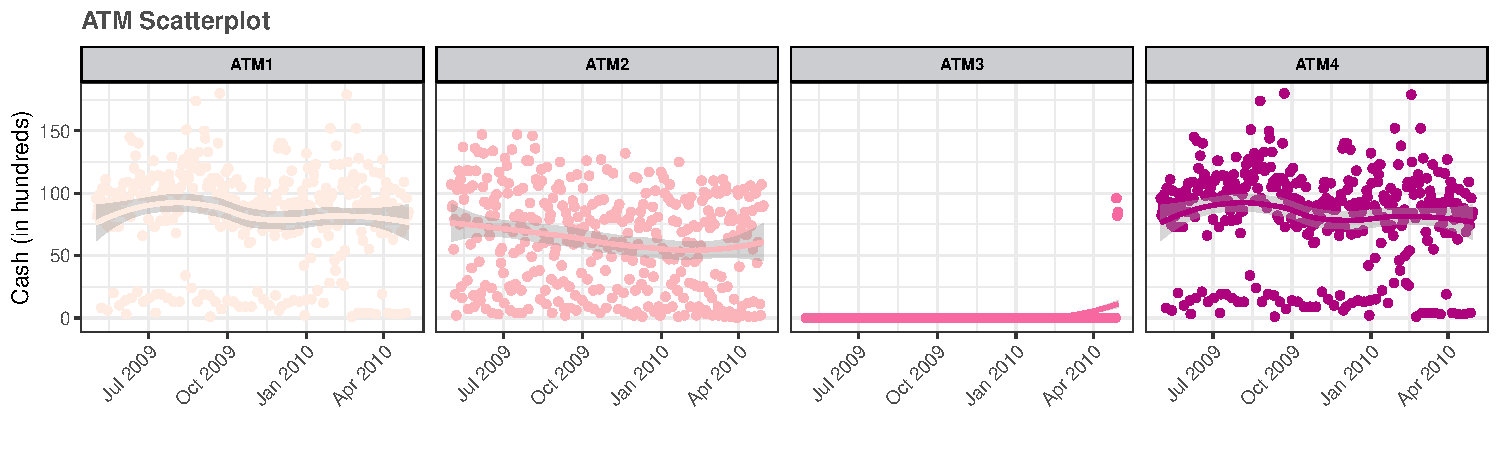
\includegraphics{Part-A-JM_files/figure-latex/unnamed-chunk-2-1.pdf}

\hypertarget{timeseries-plots}{%
\section{Timeseries Plots}\label{timeseries-plots}}

As mentioned in our data exploration, the time series for ATM3 only
contains 3 transactions, thus we deemed this series not suitable for
modeling and forecasting. As a result, our following sections focus on
evaluating, modeling, and forecasting transactions for only the ATM1,
ATM2, and ATM4 series.

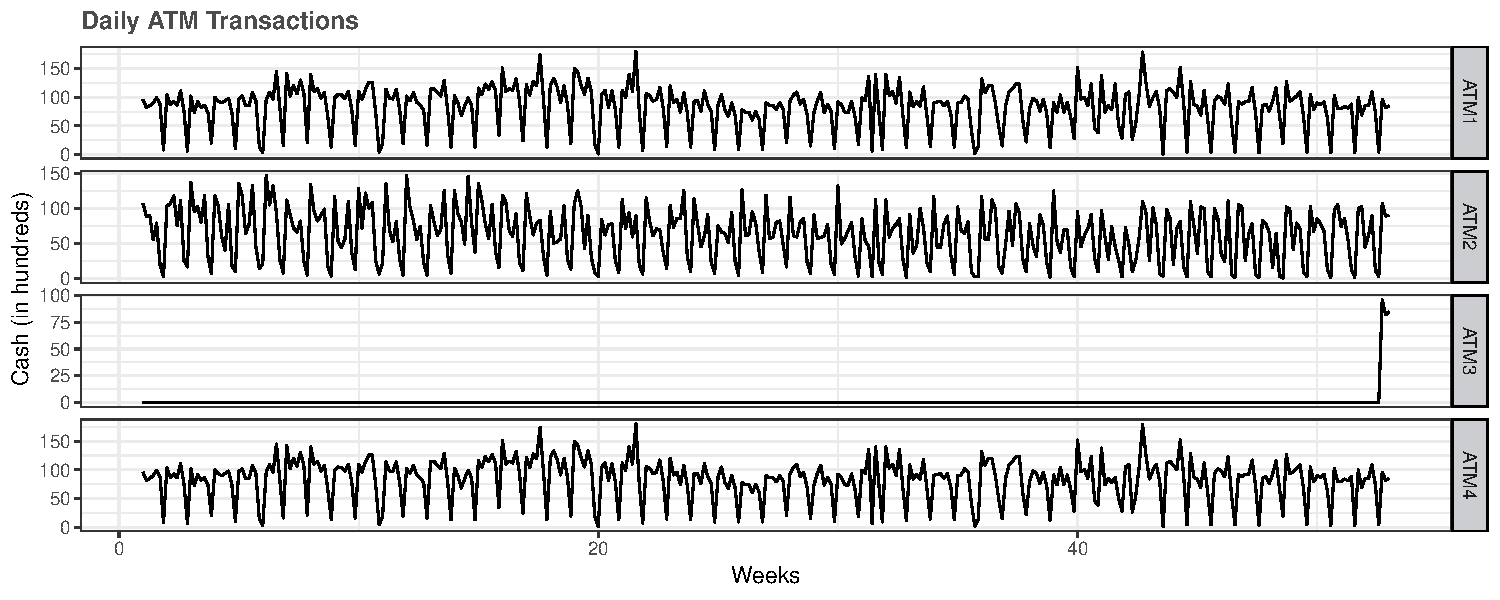
\includegraphics{Part-A-JM_files/figure-latex/unnamed-chunk-3-1.pdf}

\hypertarget{evaluation}{%
\subsection{Evaluation}\label{evaluation}}

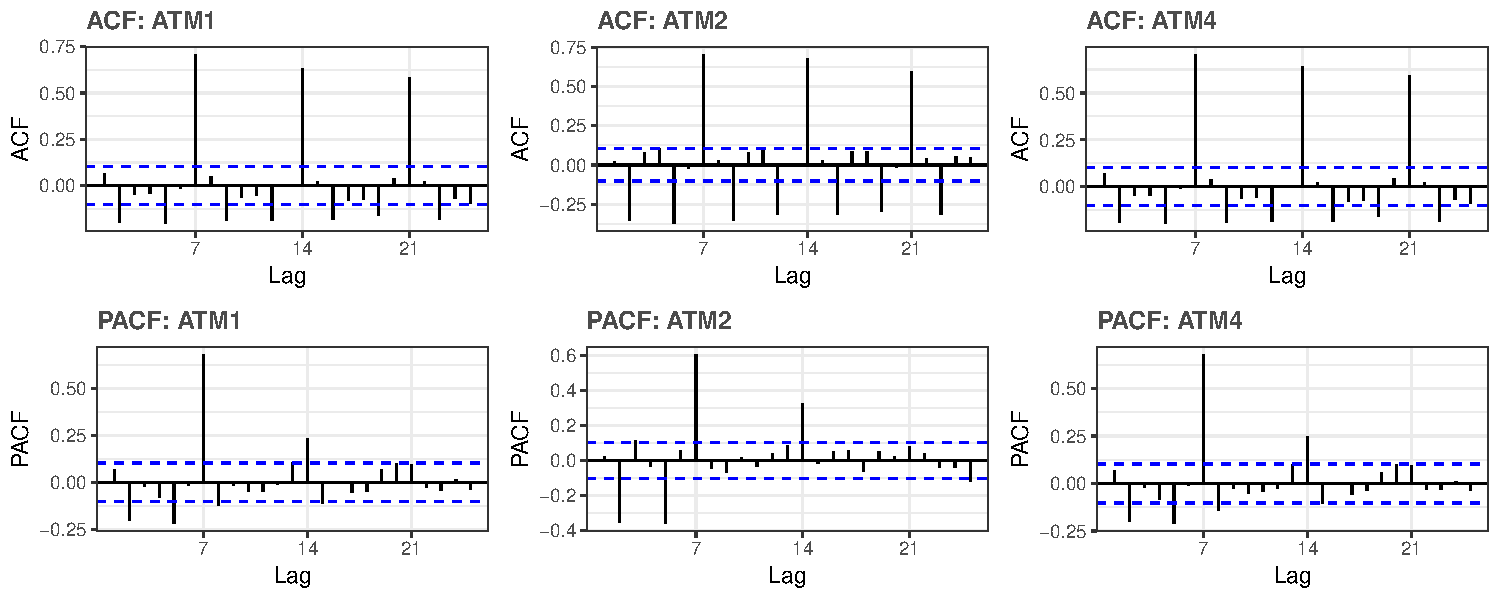
\includegraphics{Part-A-JM_files/figure-latex/unnamed-chunk-4-1.pdf}

Our ACF plots for each ATM showcases three large, decreasing lags at 7,
14, and 21. This confirms our assumption about seasonality within our
observed data as these lags are indicative of a weekly pattern. These
plot suggests our data is non-stationary, thus we performed a unit root
test using the \texttt{ur.kpss()} function and determined differencing
was required on all three series.

\begin{table}[H]

\caption{\label{tab:unnamed-chunk-5}KPSS unit root test}
\centering
\begin{tabular}{l|l|l}
\hline
\textbf{ATM} & \textbf{Root Test} & \textbf{Diff Root Test}\\
\hline
\rowcolor{gray!6}  ATM1 & 0.4967 & 0.0219\\
\hline
ATM2 & 2.0006 & 0.016\\
\hline
\rowcolor{gray!6}  ATM4 & 0.5182 & 0.0211\\
\hline
\end{tabular}
\end{table}

\hypertarget{modeling}{%
\subsection{Modeling}\label{modeling}}

We used \texttt{auto.arima()} on our differenced data to select the best
ARIMA model for our series. The following models were selected for our
series:

\begin{itemize}
\tightlist
\item
  \textbf{ATM1}: ARIMA(2,0,3) with zero mean
\item
  \textbf{ATM2}: ARIMA(1,0,4) with zero mean
\item
  \textbf{ATM4}: ARIMA(2,0,3) with zero mean
\end{itemize}

The following ACF plots show us that our differentiated data is now
stationary and the residual histograms confirm that the model adequately
fits the observed data.

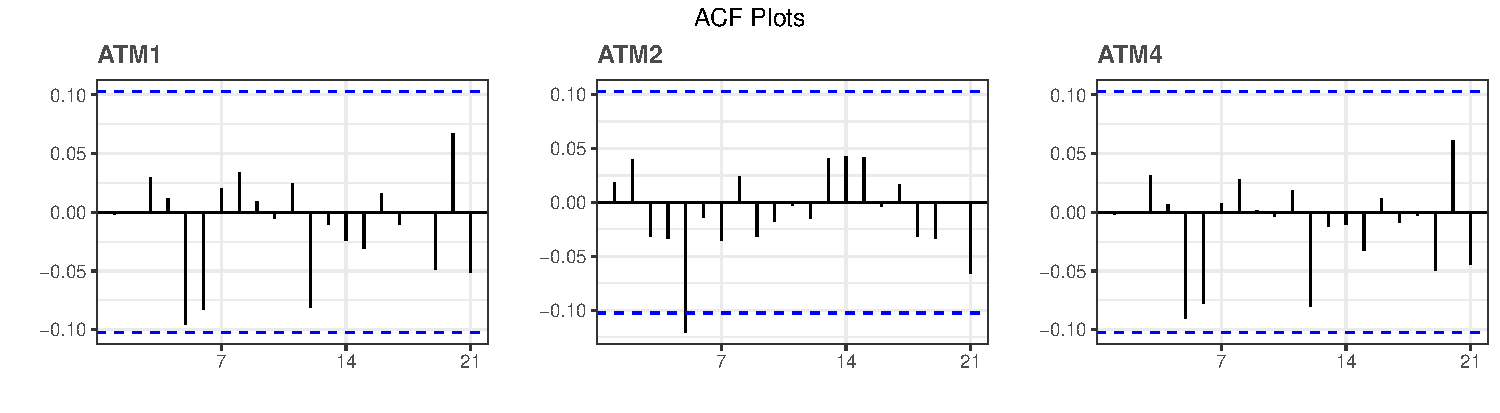
\includegraphics{Part-A-JM_files/figure-latex/unnamed-chunk-6-1.pdf}
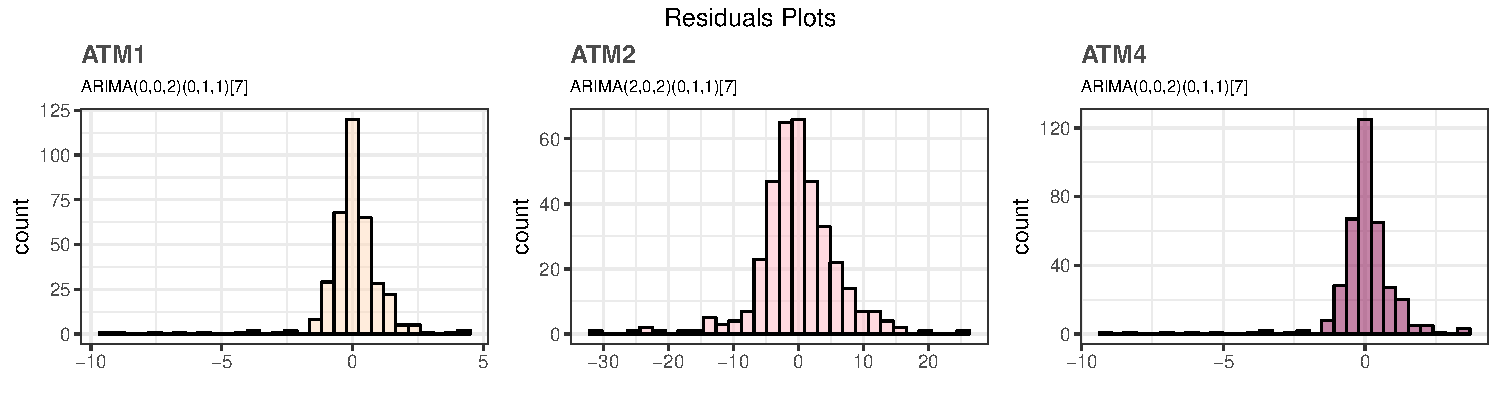
\includegraphics{Part-A-JM_files/figure-latex/unnamed-chunk-6-2.pdf}

\hypertarget{forecast}{%
\subsection{Forecast}\label{forecast}}

Finally, we applied a forecast to each series for the remaining 17 days
in May. The full forecasts can be viewed in the appendix section and are
also located within our data output folder.

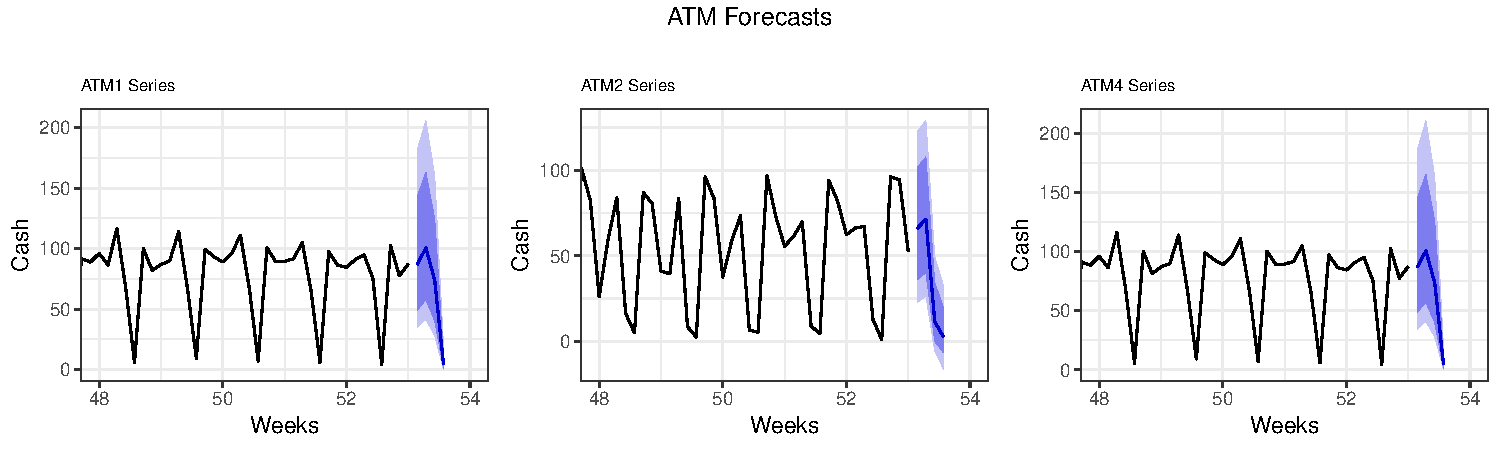
\includegraphics{Part-A-JM_files/figure-latex/unnamed-chunk-7-1.pdf}
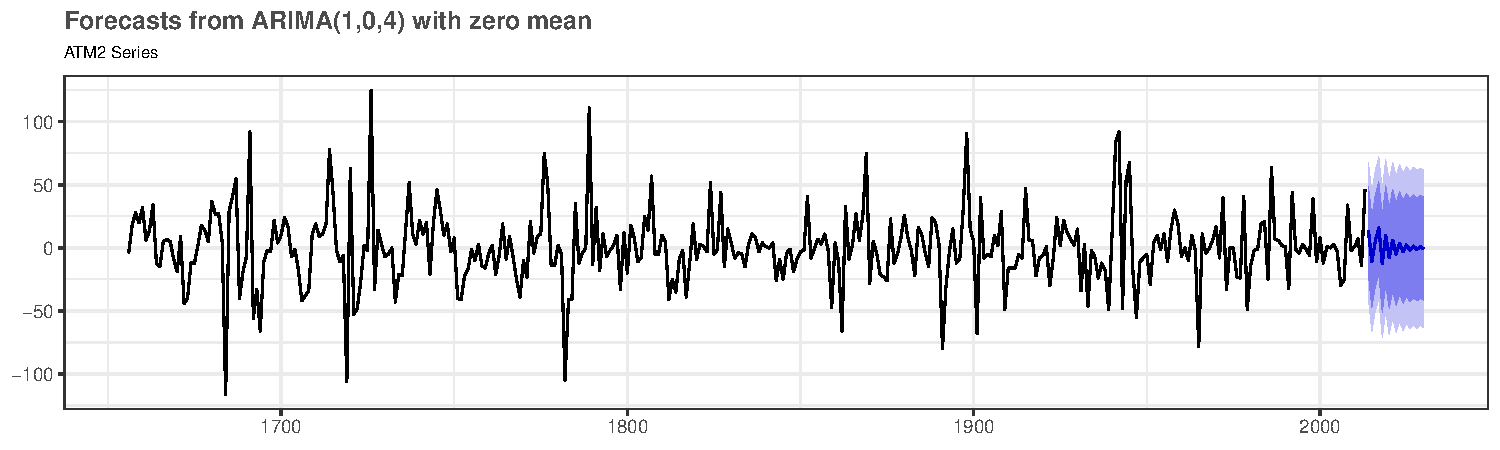
\includegraphics{Part-A-JM_files/figure-latex/unnamed-chunk-7-2.pdf}
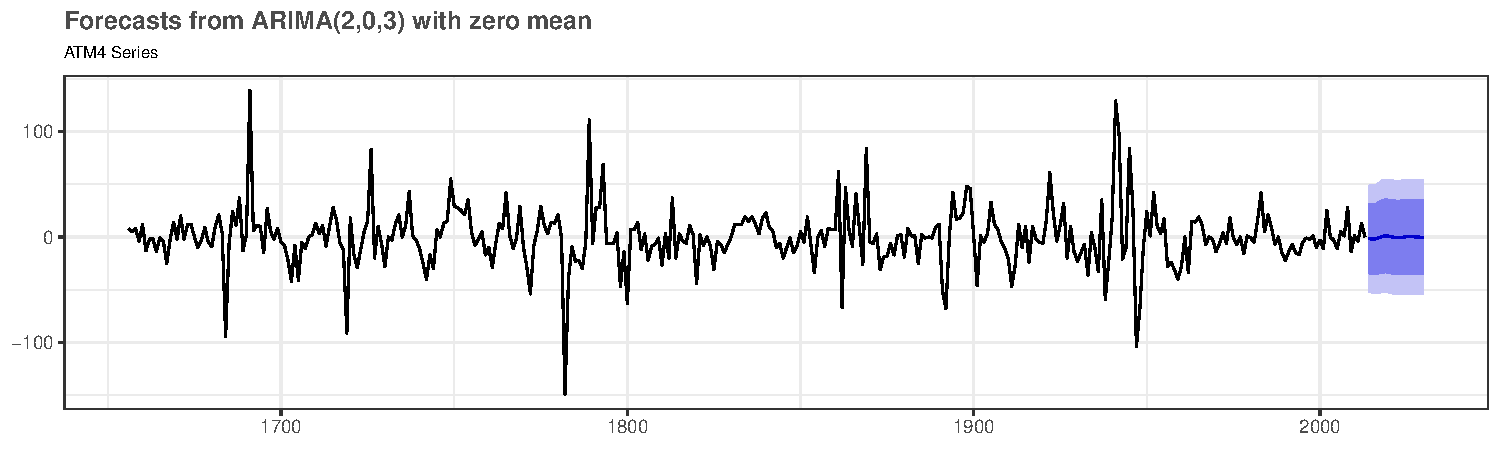
\includegraphics{Part-A-JM_files/figure-latex/unnamed-chunk-7-3.pdf}

\hypertarget{Appendix}{%
\chapter*{Appendix}\label{Appendix}}
\addcontentsline{toc}{chapter}{Appendix}

\hypertarget{Part-A}{%
\section*{Part A}\label{Part-A}}
\addcontentsline{toc}{section}{Part A}

\hypertarget{Part-A-FC1}{%
\subsection*{ATM1 Forecast}\label{Part-A-FC1}}
\addcontentsline{toc}{subsection}{ATM1 Forecast}

\begin{table}[H]

\caption{\label{tab:unnamed-chunk-8}ATM1 Forecast}
\centering
\begin{tabular}{l|r|r|r|r|r}
\hline
\textbf{ } & \textbf{Point Forecast} & \textbf{Lo 80} & \textbf{Hi 80} & \textbf{Lo 95} & \textbf{Hi 95}\\
\hline
\rowcolor{gray!6}  2014 & -1.5476468 & -34.83474 & 31.73945 & -52.45586 & 49.36057\\
\hline
2015 & -2.2246957 & -35.76049 & 31.31110 & -53.51327 & 49.06388\\
\hline
\rowcolor{gray!6}  2016 & -2.4082528 & -35.98207 & 31.16556 & -53.75497 & 48.93847\\
\hline
2017 & -0.9095920 & -35.28357 & 33.46439 & -53.48006 & 51.66087\\
\hline
\rowcolor{gray!6}  2018 & 0.7491377 & -34.21898 & 35.71725 & -52.72998 & 54.22825\\
\hline
2019 & 1.3990794 & -33.59777 & 36.39593 & -52.12398 & 54.92214\\
\hline
\rowcolor{gray!6}  2020 & 0.9070426 & -34.22027 & 36.03435 & -52.81554 & 54.62963\\
\hline
2021 & -0.0484768 & -35.41166 & 35.31471 & -54.13180 & 54.03485\\
\hline
\rowcolor{gray!6}  2022 & -0.6816097 & -36.10459 & 34.74137 & -54.85638 & 53.49316\\
\hline
2023 & -0.6624510 & -36.09316 & 34.76826 & -54.84905 & 53.52414\\
\hline
\rowcolor{gray!6}  2024 & -0.2016687 & -35.69998 & 35.29664 & -54.49165 & 54.08831\\
\hline
2025 & 0.2556483 & -35.28435 & 35.79565 & -54.09809 & 54.60939\\
\hline
\rowcolor{gray!6}  2026 & 0.4016704 & -35.13908 & 35.94243 & -53.95322 & 54.75656\\
\hline
2027 & 0.2321338 & -35.32165 & 35.78592 & -54.14268 & 54.60695\\
\hline
\rowcolor{gray!6}  2028 & -0.0427988 & -35.61500 & 35.52940 & -54.44579 & 54.36019\\
\hline
2029 & -0.2054847 & -35.78118 & 35.37021 & -54.61382 & 54.20285\\
\hline
\rowcolor{gray!6}  2030 & -0.1800679 & -35.75693 & 35.39680 & -54.59019 & 54.23005\\
\hline
\end{tabular}
\end{table}

\hypertarget{Part-A-FC2}{%
\subsection*{ATM2 Forecast}\label{Part-A-FC2}}
\addcontentsline{toc}{subsection}{ATM2 Forecast}

\begin{table}[H]

\caption{\label{tab:unnamed-chunk-9}ATM2 Forecast}
\centering
\begin{tabular}{l|r|r|r|r|r}
\hline
\textbf{ } & \textbf{Point Forecast} & \textbf{Lo 80} & \textbf{Hi 80} & \textbf{Lo 95} & \textbf{Hi 95}\\
\hline
\rowcolor{gray!6}  2014 & 13.6179414 & -21.82098 & 49.05686 & -40.58121 & 67.81710\\
\hline
2015 & -11.0244123 & -47.18551 & 25.13668 & -66.32803 & 44.27921\\
\hline
\rowcolor{gray!6}  2016 & 5.8052816 & -30.57732 & 42.18788 & -49.83710 & 61.44766\\
\hline
2017 & 15.8186530 & -21.06766 & 52.70497 & -40.59410 & 72.23141\\
\hline
\rowcolor{gray!6}  2018 & -12.4667974 & -50.90070 & 25.96711 & -71.24638 & 46.31279\\
\hline
2019 & 9.8251753 & -29.53934 & 49.18969 & -50.37765 & 70.02800\\
\hline
\rowcolor{gray!6}  2020 & -7.7432933 & -47.67490 & 32.18831 & -68.81342 & 53.32683\\
\hline
2021 & 6.1025467 & -34.17727 & 46.38237 & -55.50012 & 67.70521\\
\hline
\rowcolor{gray!6}  2022 & -4.8094622 & -45.30405 & 35.68513 & -66.74059 & 57.12167\\
\hline
2023 & 3.7903727 & -36.83704 & 44.41779 & -58.34390 & 65.92464\\
\hline
\rowcolor{gray!6}  2024 & -2.9872208 & -43.69692 & 37.72248 & -65.24733 & 59.27289\\
\hline
2025 & 2.3542508 & -38.40647 & 43.11497 & -59.98389 & 64.69239\\
\hline
\rowcolor{gray!6}  2026 & -1.8554025 & -42.64778 & 38.93698 & -64.24196 & 60.53116\\
\hline
2027 & 1.4622564 & -39.34977 & 42.27429 & -60.95436 & 63.87887\\
\hline
\rowcolor{gray!6}  2028 & -1.1524151 & -41.97665 & 39.67182 & -63.58769 & 61.28286\\
\hline
2029 & 0.9082269 & -39.92358 & 41.74003 & -61.53863 & 63.35509\\
\hline
\rowcolor{gray!6}  2030 & -0.7157803 & -41.55229 & 40.12073 & -63.16984 & 61.73828\\
\hline
\end{tabular}
\end{table}

\hypertarget{Part-A-FC4}{%
\subsection*{ATM4 Forecast}\label{Part-A-FC4}}
\addcontentsline{toc}{subsection}{ATM4 Forecast}

\begin{table}[H]

\caption{\label{tab:unnamed-chunk-10}ATM4 Forecast}
\centering
\begin{tabular}{l|r|r|r|r|r}
\hline
\textbf{ } & \textbf{Point Forecast} & \textbf{Lo 80} & \textbf{Hi 80} & \textbf{Lo 95} & \textbf{Hi 95}\\
\hline
\rowcolor{gray!6}  2014 & -1.7397027 & -35.02165 & 31.54225 & -52.64005 & 49.16065\\
\hline
2015 & -1.8523041 & -35.43051 & 31.72590 & -53.20573 & 49.50112\\
\hline
\rowcolor{gray!6}  2016 & -1.8915445 & -35.49987 & 31.71678 & -53.29104 & 49.50795\\
\hline
2017 & -0.6521306 & -35.06829 & 33.76403 & -53.28710 & 51.98284\\
\hline
\rowcolor{gray!6}  2018 & 0.6409033 & -34.40024 & 35.68205 & -52.94991 & 54.23171\\
\hline
2019 & 1.1052058 & -33.97279 & 36.18320 & -52.54196 & 54.75237\\
\hline
\rowcolor{gray!6}  2020 & 0.6860038 & -34.51254 & 35.88455 & -53.14553 & 54.51754\\
\hline
2021 & -0.0629775 & -35.49761 & 35.37166 & -54.25558 & 54.12962\\
\hline
\rowcolor{gray!6}  2022 & -0.5383252 & -36.03872 & 34.96207 & -54.83149 & 53.75484\\
\hline
2023 & -0.5063232 & -36.01206 & 34.99941 & -54.80766 & 53.79501\\
\hline
\rowcolor{gray!6}  2024 & -0.1451906 & -35.71422 & 35.42384 & -54.54333 & 54.25295\\
\hline
2025 & 0.2015531 & -35.41007 & 35.81317 & -54.26172 & 54.66483\\
\hline
\rowcolor{gray!6}  2026 & 0.3061844 & -35.30681 & 35.91918 & -54.15919 & 54.77156\\
\hline
2027 & 0.1734676 & -35.45049 & 35.79742 & -54.30867 & 54.65560\\
\hline
\rowcolor{gray!6}  2028 & -0.0343836 & -35.67590 & 35.60713 & -54.54337 & 54.47461\\
\hline
2029 & -0.1549780 & -35.80046 & 35.49050 & -54.67004 & 54.36008\\
\hline
\rowcolor{gray!6}  2030 & -0.1345348 & -35.78076 & 35.51169 & -54.65073 & 54.38166\\
\hline
\end{tabular}
\end{table}

\hypertarget{Part-A-RScript}{%
\subsection*{R Script}\label{Part-A-RScript}}
\addcontentsline{toc}{subsection}{R Script}

\begin{Shaded}
\begin{Highlighting}[]
\CommentTok{#-----DEPENDENCIES-----#}

\KeywordTok{library}\NormalTok{(readxl); }\KeywordTok{library}\NormalTok{(tidyverse); }\KeywordTok{library}\NormalTok{(janitor); }
\KeywordTok{library}\NormalTok{(zoo); }\KeywordTok{library}\NormalTok{(urca); }\KeywordTok{library}\NormalTok{(forecast)}

\CommentTok{#-----PRE-PROCESSING-----#}

\CommentTok{# load data}
\NormalTok{atm_data <-}\StringTok{ }\KeywordTok{read_excel}\NormalTok{(}\StringTok{"data/ATM624Data.xlsx"}\NormalTok{) }

\CommentTok{# clean dataframe}
\NormalTok{atm <-}\StringTok{ }\NormalTok{atm_data }\OperatorTok\StringTok{ }
\StringTok{  }\CommentTok{# create wide dataframe}
\StringTok{  }\KeywordTok{spread}\NormalTok{(ATM, Cash) }\OperatorTok\StringTok{ }
\StringTok{  }\CommentTok{# remove NA column using function from janitor package}
\StringTok{  }\KeywordTok{remove_empty}\NormalTok{(}\DataTypeTok{which =} \StringTok{"cols"}\NormalTok{) }\OperatorTok
\StringTok{  }\CommentTok{# filter unobserved values from May 2010}
\StringTok{  }\KeywordTok{filter}\NormalTok{(DATE }\OperatorTok{<}\StringTok{ }\KeywordTok{as.Date}\NormalTok{(}\StringTok{"2010-05-01"}\NormalTok{)) }\OperatorTok
\StringTok{  }\CommentTok{# ensure dates are ascending}
\StringTok{  }\KeywordTok{arrange}\NormalTok{(DATE) }

\CommentTok{## remove NA}
\NormalTok{atm}\OperatorTok{$}\NormalTok{ATM2[}\KeywordTok{is.na}\NormalTok{(atm}\OperatorTok{$}\NormalTok{ATM2)] <-}\StringTok{ }\KeywordTok{mean}\NormalTok{(atm}\OperatorTok{$}\NormalTok{ATM2, }\DataTypeTok{na.rm =} \OtherTok{TRUE}\NormalTok{)}

\CommentTok{## remove outlier}
\NormalTok{atm}\OperatorTok{$}\NormalTok{ATM4[}\KeywordTok{which.max}\NormalTok{(atm}\OperatorTok{$}\NormalTok{ATM4)] <-}\StringTok{ }\KeywordTok{mean}\NormalTok{(atm}\OperatorTok{$}\NormalTok{ATM4, }\DataTypeTok{na.rm =} \OtherTok{TRUE}\NormalTok{)}

\CommentTok{# create zoo time series   }
\NormalTok{atm_zoo <-}\StringTok{ }\NormalTok{atm }\OperatorTok\StringTok{  }
\StringTok{  }\CommentTok{# remove column & generate date in timeseries using zoo}
\StringTok{  }\KeywordTok{select}\NormalTok{(}\OperatorTok{-}\NormalTok{DATE) }\OperatorTok\StringTok{ }
\StringTok{  }\CommentTok{# generate ts using zoo }
\StringTok{  }\KeywordTok{zoo}\NormalTok{(}\KeywordTok{seq}\NormalTok{(}\DataTypeTok{from =} \KeywordTok{as.Date}\NormalTok{(}\StringTok{"2009-05-01"}\NormalTok{), }\DataTypeTok{to =} \KeywordTok{as.Date}\NormalTok{(}\StringTok{"2010-05-14"}\NormalTok{), }\DataTypeTok{by =} \DecValTok{1}\NormalTok{))}

\CommentTok{# create standard time series   }
\NormalTok{atm_ts <-}\StringTok{ }\NormalTok{atm }\OperatorTok\StringTok{  }
\StringTok{  }\CommentTok{# remove column & generate date in timeseries using zoo}
\StringTok{  }\KeywordTok{select}\NormalTok{(}\OperatorTok{-}\NormalTok{DATE) }\OperatorTok\StringTok{ }
\StringTok{  }\CommentTok{# generate ts using zoo }
\StringTok{  }\KeywordTok{ts}\NormalTok{(}\DataTypeTok{end=}\KeywordTok{c}\NormalTok{(}\DecValTok{2010}\NormalTok{,}\DecValTok{4}\NormalTok{))}

\CommentTok{#-----ATM-1-----#}

\CommentTok{#subset data }
\NormalTok{ATM1_zoo <-}\StringTok{ }\NormalTok{atm_zoo[,}\DecValTok{1}\NormalTok{]}
\NormalTok{ATM1_ts <-}\StringTok{ }\NormalTok{atm_ts[,}\DecValTok{1}\NormalTok{]}

\CommentTok{#differentiated}
\NormalTok{ATM1d <-}\StringTok{  }\KeywordTok{diff}\NormalTok{(ATM1_ts, }\DataTypeTok{lag=}\DecValTok{7}\NormalTok{)}

\CommentTok{#unit root test}
\NormalTok{ATM1_ur <-}\KeywordTok{ur.kpss}\NormalTok{(ATM1_ts)}
\NormalTok{ATM1d_ur <-}\KeywordTok{ur.kpss}\NormalTok{(ATM1d)}

\CommentTok{# ARIMA}
\NormalTok{ATM1_arima <-}\StringTok{ }\KeywordTok{auto.arima}\NormalTok{(ATM1d, }\DataTypeTok{seasonal=}\NormalTok{F, }\DataTypeTok{stepwise=}\NormalTok{F, }\DataTypeTok{approximation=}\NormalTok{F)}

\CommentTok{# Forecast}
\NormalTok{ATM1_fc <-}\StringTok{ }\NormalTok{ATM1_arima }\OperatorTok\StringTok{ }\KeywordTok{forecast}\NormalTok{(}\DataTypeTok{h=}\DecValTok{17}\NormalTok{) }

\CommentTok{# Save output}
\KeywordTok{write.csv}\NormalTok{(ATM1_fc, }\DataTypeTok{file=}\StringTok{"ATM1_Forecast.csv"}\NormalTok{)}

\CommentTok{#-----ATM-2-----#}

\CommentTok{#subset data }
\NormalTok{ATM2_zoo <-}\StringTok{ }\NormalTok{atm_zoo[,}\DecValTok{2}\NormalTok{]}
\NormalTok{ATM2_ts <-}\StringTok{ }\NormalTok{atm_ts[,}\DecValTok{2}\NormalTok{]}

\CommentTok{#differentiated}
\NormalTok{ATM2d <-}\StringTok{  }\KeywordTok{diff}\NormalTok{(ATM2_ts, }\DataTypeTok{lag=}\DecValTok{7}\NormalTok{)}

\CommentTok{#unit root test}
\NormalTok{ATM2_ur <-}\KeywordTok{ur.kpss}\NormalTok{(ATM2_ts)}
\NormalTok{ATM2d_ur <-}\KeywordTok{ur.kpss}\NormalTok{(ATM2d)}

\CommentTok{# ARIMA}
\NormalTok{ATM2_arima <-}\StringTok{ }\KeywordTok{auto.arima}\NormalTok{(ATM2d, }\DataTypeTok{seasonal=}\NormalTok{F, }\DataTypeTok{stepwise=}\NormalTok{F, }\DataTypeTok{approximation=}\NormalTok{F)}

\CommentTok{# Forecast}
\NormalTok{ATM2_fc <-}\StringTok{ }\NormalTok{ATM2_arima }\OperatorTok\StringTok{ }\KeywordTok{forecast}\NormalTok{(}\DataTypeTok{h=}\DecValTok{17}\NormalTok{) }

\CommentTok{# Save output}
\KeywordTok{write.csv}\NormalTok{(ATM2_fc, }\DataTypeTok{file=}\StringTok{"ATM2_Forecast.csv"}\NormalTok{)}

\CommentTok{#-----ATM-4-----#}

\CommentTok{#subset data }
\NormalTok{ATM4_zoo <-}\StringTok{ }\NormalTok{atm_zoo[,}\DecValTok{4}\NormalTok{]}
\NormalTok{ATM4_ts <-}\StringTok{ }\NormalTok{atm_ts[,}\DecValTok{4}\NormalTok{]}

\CommentTok{#differentiated}
\NormalTok{ATM4d <-}\StringTok{  }\KeywordTok{diff}\NormalTok{(ATM4_ts, }\DataTypeTok{lag=}\DecValTok{7}\NormalTok{)}

\CommentTok{#unit root test}
\NormalTok{ATM4_ur <-}\KeywordTok{ur.kpss}\NormalTok{(ATM4_ts)}
\NormalTok{ATM4d_ur <-}\KeywordTok{ur.kpss}\NormalTok{(ATM4d)}

\CommentTok{# ARIMA}
\NormalTok{ATM4_arima <-}\StringTok{ }\KeywordTok{auto.arima}\NormalTok{(ATM4d, }\DataTypeTok{seasonal=}\NormalTok{F, }\DataTypeTok{stepwise=}\NormalTok{F, }\DataTypeTok{approximation=}\NormalTok{F)}

\CommentTok{# Forecast}
\NormalTok{ATM4_fc <-}\StringTok{ }\NormalTok{ATM4_arima }\OperatorTok\StringTok{ }\KeywordTok{forecast}\NormalTok{(}\DataTypeTok{h=}\DecValTok{17}\NormalTok{) }

\CommentTok{# Save output}
\KeywordTok{write.csv}\NormalTok{(ATM4_fc, }\DataTypeTok{file=}\StringTok{"ATM4_Forecast.csv"}\NormalTok{)}
\end{Highlighting}
\end{Shaded}


\end{document}
